\chapter{Background}\label{ch:Background}

\begin{mynote}
%\vspace{0.5cm}
\subsubsection{Chapter outline}
In this chapter, I review previous literature on which I build my research on expenses tasks in a financial office setting. The first half of the chapter will focus on the setting, and discuss challenges of performing tasks in an office environment. The second half of the chapter will focus on the data entry task, and how certain design changes can influence people's speed and accuracy. 
%\vspace{0.2cm}
\end{mynote}

\section{Terminology}
Throughout the thesis, I use the key terms inquiries, interruptions, time cost and information access cost. To avoid confusion, I clarify the definitions of these terms here.

\textit{Inquiries} are a type of self-interruption, and happen when a person goes away from a task, to look up information that aids the completion of that primary task \citep{Jin2009}. This type of interruption is the main focus of the thesis. In sections where the terms \textit{interruptions} or \textit{self-interruptions} are used, rather than inquiries, it can be assumed this section refers to all types of interruptions. 

\textit{Time costs} refer to the time involved to complete an action. Prior studies in cognitive psychology have used the term \textit{information access cost}, which  is a particular type of time cost, and refers to the time, physical and/or mental effort required to access information \citep{Gray2006}. Because this thesis looks at a broader definition of time costs to look up information, which can be caused by accessing information, but also searching for information and getting distracted by other information, the term time costs is used for the majority of the thesis. When the term information access cost is used, usually when discussing prior work, it refers to the specific time cost of accessing information. 

\section{Interruptions and fragmentation of work}
%Occurrence of interruptions
Computer work frequently gets interrupted: on average, office workers either get interrupted or self-interrupt every three minutes \citep{Gonzalez2004}. People switch between tasks, but tasks themselves are also often fragmented: people have to switch between documents and applications to look up information for their task. Some interruptions can be beneficial: for example, getting the right information can have a positive impact on work \citep{Jin2009}, and short breaks can improve mood and restore energy \citep{Mark2014a}. However, frequent or longer interruptions can reduce productivity, and both controlled and in-the-wild studies have found a link between fragmented attention and a decrease in work performance \citep{Bailey2001, Carrier2015}. 

Office workers change their main work activity on average once every 11 minutes \citep{Mark2005}, and reportedly switch between tasks 50 times over one work week \citep{Czerwinski2004}.  Users can leave the primary task interface because they are distracted by a notification or because they deliberately decide to switch to a completely other task, but can also leave to look up task-relevant information. The subtask of looking up information is relevant to the primary task so may not always be labelled as an interruption from the main activity, but resuming the primary task of entering information can still be difficult \citep{Rule2013}.

\subsection{Why and how do people interrupt?}
To understand some of the reasons and underlying mechanisms of interruption behaviour, interruptions have both been studied through field studies and controlled experiments.

%more in afternoon, when bored
Field studies have been done to understand interruptions in a situated settings such as healthcare \citep{Grundgeiger2010} and office environments \citep[e.g.][]{Czerwinski2004, Gonzalez2004}. 

\citet{Jin2009} conducted a observational study of self-interruptions during computer tasks. They identified seven categories of self-interruptions: adjustments, breaks, recollections, routines, triggers, waits, and inquiries. Adjustments happen when people try to adjust and improve their work environment, for example by closing irrelevant documents. Breaks are moments when people switch to something else because they want to take a rest from the main task. Recollections occur if people remember they need to perform another task. Routines are self-interruptions that happen out of habit, such as checking social media regularly. A trigger is an external stimulus that triggers the user to switch to another task. Waits are when people switch to something else during a delay in the primary task. Lastly, an inquiry, which is the type of interruption we focus on in this paper, happens when a person goes to look up information to aid the completion of a primary task. Though in Jin and Dabbish’s study inquiries positively impacted participants’ work because they quickly found what they needed, Jin and Dabbish speculate that this behaviour may be disruptive and distracting if information cannot be found straight away.

An interview study on interruption management strategies found major differences in the level of difficulty for users to manage external versus self-interruptions.  Whereas external interruptions may be ignored or deferred, self-interruptions require more self-control, and are experienced as harder to resist and as more distracting \citep{Kim2017}. Furthermore, self-interruptions take more time to recover from than external interruptions as they can end up taking much longer than planned. When switching between computer windows, there are numerous opportunities to get distracted and get diverted from the main task. For example when switching to communication tools, users can get tempted to answer unrelated messages instead \citep{Mark2012}. %The longer an interruption is, the more disruptive it can be, so it is important to manage time spent on interruptions from a task.

There are also individual differences in people's tendency to attend to distractions and to resist interruptions \citep{Mark2016a, Lyngs2018}. \citet{Mark2016a} conducted a field study with office workers, in which window switching behaviour was measured, and participants were asked to fill in a personality survey at the end of each day. They found a positive relationship between how people score on a Neuroticism and Impulsivity scale, their switching behaviour, and how productive they felt at the end of the day. They conclude that distractibility could be a personal trait. 

%External interruptions
A limitation of field studies is that it is difficult to link factors that may influence the occurrence of interruptions, and measure its effect on task performance. Controlled experiments are a suitable method to study some of the mechanisms influencing interruptions and task performance. 

%Length of interruption

%Let people wait before resuming task.
In an experiment by \citet{Brumby2013}, people had to perform a data entry task and were interrupted several times to do a secondary task. They manipulated the cost of making an error and if the cost was high, an error would cause the participant to be locked out for 10 seconds before they could resume the primary task. In this condition, people took a longer time to resume, but were less likely to make errors. A lockout made people adopt a memory-intensive strategy and take the time to remember where they were in the sequence before resuming the task. 

%
%Timing of interruption
In these studies, the researchers enforced an external interruption that participants had to respond to. \citet{Salvucci2010} investigated how people manage interruptions which they can defer. They found that  


\subsection{Interruption management tools}
There have been different approaches to support self-interruption management and improve people's focus. 

%Giving reflective information
Commercial applications, such as RescueTime and ManicTime, provide users with an overview of all their computer activities, to increase awareness of their use of time. Users can view how much time they spent in particular documents, websites and applications, and during which hours of the day. Little work has evaluated how effective these applications are in improving focus, and interview studies have reported a lack of engagement among users \citep{Collins2014, Whittaker2016}. An interview study by \citet{Collins2014} on understanding people’s use of RescueTime found four barriers to explain people’s lack of engagement with the data: the data lacks salience, a lack of context made it difficult to extract work patterns from the data, participants felt it was not a true representation of their actual activities, and they were not sure what actions to take based on the data. 

\citet{Whittaker2016} interviewed office workers and students to establish user requirements for a time awareness application, and found users were primarily interested in their current activities rather than long-term behaviour. Therefore, they developed and evaluated an application which presented users with a visualisation of the last 30 minutes of computer activity. The application reduced the time spent in email, browsing and social media, but it did not increase time spent on work and it was unclear whether it improved people’s productivity. Whittaker et al. speculated that participants may already have time limits to spend on work, but are more flexible with the amount of time they spend on other online activities.

%Blocking distractions
Other commercial tools such as StayFocusd, Freedom and FocusMe limit access to specific sources. \citet{Kim2017} developed an intervention that allowed people to block applications and websites across devices for a fixed period that they considered distracting. The blocking feature was viewed positively by participants who found it difficult to mitigate self-interruptions themselves. However, many distracting sources, such as web browsers and instant messaging applications, can not be blocked during work because these need to be accessed for the current work task. To investigate how appropriate a blocking approach would be in the workplace, \citet{Mark2018} conducted a field study with office workers using blocking software for one week. Participants installed software that allowed them to disable websites, and were asked to block any websites they considered distracting and nonessential to work. Several participants disliked the feeling that the software was controlling them, and rather wanted to learn how to gain control themselves over their work and interruptions.

Other interventions suggest giving participants information during a specific task may help focus. \citet{Gould2016a} looked at people’s switches to unrelated activities during an online data entry task. They found that an intervention that encouraged people to stay focused after they had self-interrupted reduced the number of switches to unrelated tasks. 

\subsection{Summary}
Interruptions in the workplace are common, and both controlled and field studies have found a link between fragmented attention and a decrease in work performance \citep{Bailey2001, Carrier2015}. Various tools have been developed aiming to reduce interruptions and digital distractions, but there 


\section{Managing information needs}
%\subsection{Occurrence of looking for information}
Increased screen space allows people to have more windows open at once. This may reduce the need for people to open and close windows and hold information in memory when flicking between windows, but the responsibility stills lies with the user to first collect and organise all the required resources for the task \citep{Bardram2006}. Some task management applications have been built to support users to collect and group information needed for the task, but people often do not know the complete context of their activity yet and the information they will need. In addition, manually categorising and grouping task-related information can be time-consuming \citep{Cangiano2009}.

People do not always realise they need certain information until they have started a task. Leaving the primary task interface to look up this information does not have to be bad if it is useful for the current activity, but resuming the primary task after this interruption still takes time \citep{Rule2013}.
\citet{Sohn2008} conducted a diary study to get an insight in people's information needs on mobile phones and how they address these needs. They did not focus on a particular task, but asked participants to keep a record of all instances where they needed information for an activity they were doing.

The information needed was retrieved from both public and personal sources on their mobile phones, such as website and e-mails, as well as physical locations. Four main factors determined whether participants looked up the information when they needed it, when they addressed it later or when they did not address it at all: urgency, importance, cost, and situational factors. The more urgent and important it was to have the information for the activity they were doing, the more likely it was they looked up the information at the moment they realised they needed it. The more time or monetary cost was associated with getting the information, the more likely they were to not address it or leave it until later. Other reasons for looking it up later or not at all, was that they were currently involved in an activity that made it difficult to address the information need at that moment, or they did not know where to get the information from.

People sometimes had to switch between several information sources and applications for one task, such as personal e-mails, search engines, and Google Maps. The more effort and time it took to go in and out of these several sources, the more likely it was that the participant gave up on looking up the information at that moment and deferred it until later. The source where people needed to get the information from, and how costly it was to access this source, also influenced whether people looked up information as they needed it or not.

The authors conclude mobile devices should take into account the activity people are doing to make sure information related to a task becomes easy to access. Though it may be difficult to predict which information will be needed, it should be at least easier for users to switch between different information sources.

The information needs in this study were primarily for personal rather than work activities, and people may be less flexible in deciding to not look up information at all when it is work-related. They may however decide to look up information later, and if it is costly to access information or depending on importance of accuracy or efficiency, decide to rely on information they have memorised rather than looking up the information of an external source. 

\subsection{How do people manage information needs?}

\subsection{Information management tools}
Most computer applications are designed to support a part of a task, but do not consider that users may have to use multiple applications for the same activity \citep{Cangiano2009}. Several studies on office workers have found that information work often does not happen within one application or document, but can be highly fragmented \citep{Cangiano2009, Czerwinski2004, Mark2005, Sellberg2014}. People have to go in and out of several applications \citep{Cangiano2009, Iqbal2007}, switch between tasks \citep{Czerwinski2004, Mark2005}, and have to coordinate information distributed over paper files, electronic databases, e-mails, as well as people \citep{Sellberg2014}. 

Office workers are dealing with an increasing amount of information, and may have to leave the task interface frequently to look up information. As discussed earlier, hiding information and increasing access costs may have a positive effect, as people encode the information better in memory. They do not need to look up the information as frequently and are more efficient in completing the task \citep[e.g.][]{Waldron2011}. Having the information well-memorised can also make people more robust against interruptions \citep{Morgan2009} and showing data in a harder-to-read font can make people more accurate in text and number transcription tasks \citep{Soboczenski2013}.

In these studies the information to hold in memory was limited and came from one source. When dealing with a lot of information from multiple sources, decisions on what has to be presented where and in what manner is still a challenge and it is often up to users to arrange the required resources for the task \citep{Bardram2006, Grudin2001}.

Flipping back and forth between several documents can make you lose train of thought, and when interrupted you may have forgotten the original intention of what you intended to look up \citep{Grudin2001}.  In order to help people manage information and minimise switching between windows, both multiple and larger screens have been introduced into the workplace. While a number of studies have favoured one large screen over two smaller ones \citep[e.g.][]{Bi2009}, the two solutions seem to have different benefits.

\citet{Bi2009} conducted a study comparing people's behaviour in office work when they had to use one small screen, two small screen, and one large screen. People arranged information on their available screen space differently in each condition. For two screens, people dedicated one screen for their primary task which filled up the entire screen. They moved all information they did not need at the moment to the second screen and did not bother re-arranging the windows: they would only attend to the second screen when they needed information, and deliberately allocated the second screen for a different purpose than the first screen. For one large screen, participants first spent a certain amount of time optimising the layout of the windows by resizing and re-arranging them. They put all windows needed for the primary task in the center of the screen and placed other windows in the periphery.  As participants needed information from this periphery, they dragged the window to the center of the screen rather than interacting with that particular part of the screen. On the other hand, if participants needed information from the second screen, they physically turned to the second screen and interacted with it but did not drag the information to the primary screen, unless they had to interact with it for a longer time.  

For the majority of tasks, participants preferred one large screen over two screens, as it made them feel more immersed in, and surrounded by, their work. Two screens had a physical distance between them, so large documents could not easily be seen across the screens. A further drawback from having two screens was that it needed more physical space on a desk. \citet{Bi2009}  mentioned that a large screen made people better able to monitor other applications during work, such as emails. This was viewed by the authors as a benefit, but may also be more distracting. If such applications are instead placed on a second screen, people will be less disrupted by them because their visual attention is not there, but they can still easily glance at it to see if there are any new notifications \citep{Grudin2001}.  

Despite the popularity of one large screen, \citet{Grudin2001} states dividing screen space up in multiple monitors can sometimes be better. He argued that the main benefit of having a second screen is not so much the increase in screen space, but the partitioning of information into dedicated areas. He compares screen size with a house: sometimes it is better to have two rooms rather than one big room, as you can use the rooms for different purposes, such as one for a bedroom and one for a living room. Similarly, having multiple screens prompts people to think more about where to put which information. To support his argument, he conducted a field study looking at how office workers use multiple screens to arrange information. Participants positioned information they did not need at the moment on a second screen where they were not distracted by it, but could easily access it when needed. People preferred that information was always in the same known location and referred to the second screen whenever they needed to look information up, even when they were aware they could also access it using their primary screen as well, where the information was sometimes less time-consuming to access \citep{Grudin2001}. 

A larger screen can better support people in multitasking, as people will not need to flick back and forth between windows as often, but can have these open and on the screen simultaneously \citep{Czerwinski2003}. However, it can also have a snowball effect: as screen size increases, so does the number of open windows, and people engage in more complex multitasking \citep{Robertson2005}. In addition, a large screen may reduce having to click and tab between windows but it can introduce another type of access cost, which \citet{Robertson2005} refer to as the \textit{'distal information access cost problem'}: as screen size increases, it becomes harder and more time-consuming to target and select certain buttons and windows. 

\subsection{Task and information management}
To make it easier to re-find documents for a particular activity, some systems have looked at grouping windows and documents. For example, TagFS (source) allows users to tag documents and define groups. GroupBar (Smith et al., 2003) makes it possible to group windows needed for a task in the task bar. This can be particularly useful when resuming an interrupted task: the user can see which documents were used before leaving the task.
These tools offer the user flexibility in organising information sources in different ways, but come with a number of limitations. First, it assumes the user knows in advance what information is needed for which purpose. While some information needs are known in advance of the data entry task, it regularly occurs the user needs unexpected information. Second, categorising documents can be time-consuming, and people are often not willing to invest time doing so (source). Especially for data entry tasks where documents are only briefly needed, people may not make the effort to group information. Lastly, studies have shown that when people do make the effort to organise documents into groups, they often use inconsistent labels, making it difficult to re-find information later (Jones, Jiranida Phuwanartnurak, Gill, \& Bruce, 2005). 

\subsection{Information search}
In addition to information management, other studies have focused on supporting information search. An issue with looking for information is that information can be scattered across applications, and users have to go in and out of these separately to search and find what they are looking for. To support re-finding information across different applications, Dumais et al. (2003) presented a tool called Stuff I've Seen. Users were presented with a unified search interface which they could use to search through information they had already seen before, such as emails and web pages. A user study, where participants installed the tool on their computer and used it for two weeks, showed that users used the search tools of individual applications less frequently and used Stuff I've Seen instead. The focus of the tool was to improve search, rather than the scheduling or reducing of interruptions from work to search. The user still had to switch from their main task environment to a separate tool, and create a search query or use filters to view relevant search results. People do not always know what to search for, as demonstrated by both previous literature (source) and Study 2 of this thesis. Furthermore, for familiar documents, the preferred way of navigation is often browsing, rather than searching (Bergman, Beyth-Marom, Nachmias, Gradovitch \& Whittaker, 2008).
Whereas Stuff I've Seen only supported searching for digital information, PimVis was developed by Trullemans, Sanctorum, \& Signer (2016) to allow search across both paper and digital sources. A graphical user interface presented a visualisation of documents, grouped according to the context in which they are relevant. Bookcases and filing cabinets were augmented with LEDs, which would light up if users selected a document in PimVis that was contained in these physical locations. By opening a document in PimVis, the user could see documents related to this document. PimVis was evaluated using the task of finding documents for writing a paper. As PimVis was a standalone application, users had to switch away from their current application, such as their text editor, and open the document in PimVis to view its related documents. Participants reflected that PimVis would be useful for archived documents. For so-called 'hot' documents, which are needed for short-term tasks in the moment, they would value seeing related documents in the environment they are currently already working in, rather than having to go to a separate application. In the user study, the grouping of documents as well as augmentation of physical artefacts were set up by the researchers. The primary aim was to see whether participants could easily navigate through PimVis. They were given tasks to find specific documents, such as 'You want to read the paper called X, which is related to the paper called Y'. In practice, the user would have to pre-define in which contexts documents were to be used and how they were related to other documents, which has the same drawbacks as categorising and labelling documents as discussed above.

\subsection{Interruptions and delayed intentions}
One reason why people are not always able to organise information efficiently is because they may not know they need information until they have started a task. In Study 2, participants disrupted their data entry work as soon as they realised they needed certain information. Prior work on self-interruptions found that office workers often start new tasks before completing old ones (Czerwinski, Horvitz, \& Wilhite, 2004; Jin \& Dabbish, 2009). If  people are able to keep track of tasks they need to perform, it may help them in deferring these tasks until a more convenient moment, rather than addressing them as they realise they need to be done (Jin \& Dabbish, 2009). For example, an interruption between subtasks is less disruptive than an interruption in the middle of a subtask (Bondarenko, 2010; Gould, 2014).
Gilbert (2015) looked at people's off-loading behaviour in both an experimental and naturalistic setting. Participants had to remember to perform an action later, and had the option to offload this intention or to keep it in memory. In both settings, a majority of participants offloaded these intentions when they had the option, and this significantly improved their performance. Additionally, in Study 3 of this thesis, where participants had to remember which blocks to drag to which location, a selection of participants placed blocks nearby what they though the correct location was, to not have to remember its location, and as a reminder to place them there later. 
These findings suggest that if people have to memorise which information to retrieve, they may benefit from options to offload these information needs, and are able to effectively defer information subtasks until a convenient moment in the main data entry task. 

\subsection{Documents at hand}
Bondarenko \& Janssen (2005) compared how information workers store paper and digital sources. One user need they found was that documents should be embedded in task-related context information, as it helps to resume a task after an interruption. In addition, in Bi \& Balakrishnan's (2009) study on large and multiple display use, office workers felt more focused on the task and immersed in their work when surrounded by task-relevant documents. A limitation of most tools discussed so far is that the task window and information window are separate, and users need to switch between these. Microsoft Office's new feature TAP instead is a built-in add-on, which allows users to place relevant documents in a task pane next to their working document. The aim of the feature is to keep focus on document creation, rather than looking up information. The feature is presented as a task pane within a document, such as a text document or email, and contains an overview of documents that may be relevant to the current document. The task pane initially shows files that are most frequently used. If the pane does not show the documents that the user is looking for, there is also a search option within the task pane. 
The feature can reduce interruptions from the task interface. However, the TAP feature is application-specific: the user is only able to include other Office documents, and not information sources such as websites and databases. Furthermore, it is mainly focused on re-using content from archived documents, and assumes the user knows which documents to re-use. It may be less suitable for situations where people do not know where to get information from.  
 
\subsection{Type of activity}
An important difference between previous work on information management and the studies in this thesis is the nature of the activity studied. Bondarenko \& Janssen (2005) distinguish between two types of activities that information workers engage in: research activities and administrative activities. For an administrative activity, users go in and out of a variety of documents rapidly. For research activities, users need a smaller variety of documents, but these are needed for a long time. The tasks studied in most information management studies were more similar to research activities: participants had to read information to improve their understanding of a legal case (Cangiano \& Hollan, 2009), or they needed to have the information for a longer time during a task (O'Hara, Taylor, Newman, \& Sellen, 2002). A data entry task however is more similar to an administrative task. This distinction in activities is important, as it influences people's information collection strategies (Bondarenko \& Janssen, 2005), and whether design considerations from previous work are applicable. Participants may not want to spend effort to organise information, such as grouping them and indexing them, if they only need the documents briefly. On the other hand, having contextual information nearby can be beneficial for both types of tasks, as it minimises interruptions and holding items in memory.

\subsection{Time management applications}
In order to improve focus and mitigate self-interruptions, Kim, Cho and Lee (2017) developed an intervention that allowed people to temporarily block specific sources that they considered distracting, such as email, IM applications and social media. However often these sources then needed to be accessed after all for the task they were working on. Other commercial applications do not block sources but instead provide users an overview of their computer activities, to reflect how much time they spend in total on tasks, and certain sources ("ManicTime," 2018, "RescueTime," 2018). However, as these tools provide information of past usage, it is often not clear to users what they have to do with the data (Collins, Cox, Bird, \& Cornish-Tresstail, 2014), and there is little evidence of their effectiveness in improving focus (Whittaker, Hollis, \& Guydish, 2016). Gould, Cox and Brumby (2016) looked at switching behaviour during online crowdsourcing work, and found that an intervention during work that encouraged people to stay focused after people had interrupted reduced number of switches to unrelated tasks. Recognising that switches occur as part of the task, we consider whether the duration of switches can be reduced by giving people real-time feedback on how long they switch away for during a data entry task. This is important to consider, because the longer people interrupt, the more disruptive it is (Monk, Trafton, \& Boehm-Davis, 2008), and the harder it is to resume a task (Altmann, Trafton, \& Hambrick, 2017).

\subsection{Summary}
Office work can be highly fragmented, and people have to go in and out of several documents, applications and windows for the same activity. It is often up to the user to collect information, and it should be made easier for people to collect information for a task and resume it when they leave the primary task interface to look up information. The cost to access information, the urgency and importance of an information need, and the current situation people are in influences their decision on whether they look up information as they need it or not. 

Office workers deal with an increasing amount of information and it is challenging to decide how to present information needed for the task. An increased screen size can reduce certain access costs, such as mouse clicks to flick back and forth between windows, but may introduce other access costs, such as time to select the right window. 
Multiple and larger screens both increase screen space, but people adopt different behaviour and strategies for each set-up. Two monitors makes people dedicate a second screen for all information sources and secondary tasks, so they can focus their attention on one screen. When using one large screen, people will re-arrange windows to have more windows open at the same time and focus on the primary task but still be aware of other windows. 

\section{Data entry}
%Occurrence of data entry
While prior work has studied the phenomenon of fragmented office work and self-interruptions during computer activities, it has generally not focused on a specific task. A core computing task in office scenarios is data entry. An example of a data entry task is completing a payment request form, in which information has to be entered into specific fields of the form, such as the person’s name, address, and bank account details. Interruptions
during this type of task can be particularly disruptive as it not only takes time to resume the task, but it can also increase data entry errors. Numerous lab-based experiments have been conducted that demonstrate how changes to the data entry interface can influence people’s strategies and reduce errors.

\subsection{How do people perform data entry tasks?}
A data entry task can be broken down in four stages (see Figure \ref{fig:ch2_hip}). An information source contains the input, i.e. the data to be entered. In the perception stage, the user perceives this data. In the encoding stage, the user encodes these in the mind. In the execution stage, the user enters them into a device which produces the output of the task, namely the data entered. Additionally, there can be a checking stage where the user checks their entered output against the original input to see if it matches.

\begin{figure}[!ht]
\centering
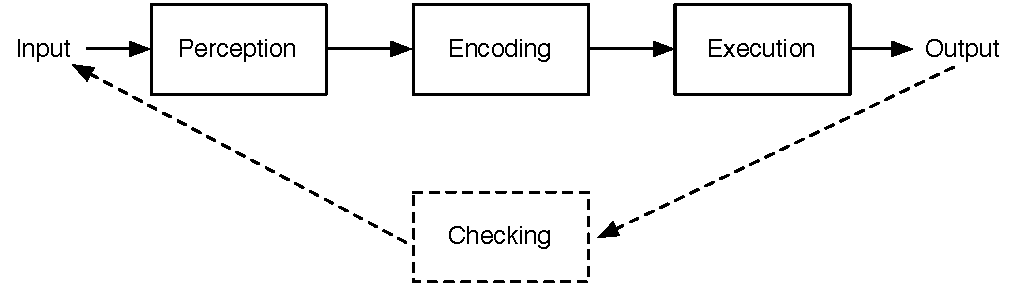
\includegraphics[width=0.8\textwidth]{images/background/HIP.pdf}
\caption[Different stages of a data entry task]{The different stages of a routine data entry task: a user perceives data input, encodes these in the mind, executes certain actions to enter data and produce the output, and can check the output against the original input.}
\vspace{-3pt}
\label{fig:ch2_hip}
\end{figure}

The following four sections will describe each stage of the task in turn, and will discuss research that has been done to reduce errors at this stage. 
Throughout this thesis the terms data, text, and number entry are used. If data is used, this refers to alphabetic, alphanumeric, and numeric characters. 
If the term text is used and no particular clarification is given, this refers to alphabetic text. If numbers are discussed and no specification is given, this refers to the Arabic notation of numbers, in other words digits. 

\subsubsection{The perception stage}
A data entry task begins with the user looking at the data that has to be entered on a data source.
Both the design of the data source as well as the data itself can ultimately have an influence on task performance. In this section, I will describe the following themes: the distribution of internal and external cognition, external representations, the memorability of data, and how presenting data in a disfluent manner can influence people's cognitive encoding of the information.

\subsubsection{Distributed cognition}
When people perform a task, they can make use of information in their mind, or retrieve information from the external environment \citep{Norman1993}.
The distributed cognition approach has been used as a theoretical framework to explain how people make use of internal and external information to carry out work \citep{Hollan2000}. In contrast with traditional cognitive science approaches that take the individual mind at the center of analysis, distributed cognition explains how the completion of a task is determined by one or more users interacting with each other, their environment, as well as external artefacts \citep{Hutchins1995}. The framework suggests that external representations are not merely a memory aid to off-load the limited capacity of someone's working memory, but form an integral part of cognition. In other words, it is not only the amount of external information, but also its format that can considerably affect performance \citep{Gong2009, Zhang2009}.
To be able to understand how people work, it is not enough to know how the mind processes information but it is also important to know how the information is arranged in the physical world \citep{Hollan2000}. 

\citet{Payne2013} argue that some proponents of distributed cognition assume people off-load as much cognition to external resources as possible. However, as will be discussed in section \ref{sec:Encoding_stage}, the decisions people make on whether to offload or not is better understood as adaptive, and is affected by context as well as the design of the interface or artefacts. 

\subsubsection{External representations}
Building on the work that external representations are part of cognition and that their format influence how people process and understand information, work has been carried out to explore different ways to represent information to the user. 

An important factor in designing appropriate external representations is to consider how users currently use these representations. \citet{Hutchins1995} gives a case study of cockpits as an example, in which the dial to indicate airspeed was replaced with a more precise digital display. This design did not take pilots into consideration, and only after interviews was it revealed that the new display did not match with how pilots made use of this external information. Pilots did not think of the speed as a number, but used the spatial structure of a dial to perceive their current speed and its proximity to the desired speed. By replacing the dial with digits, they lost this information. 

With a better understanding of how people use representations in a certain context, these representations can also be organised in a way to make people adapt to more desirable strategies. \citet{Back2013b} looked at programming infusion pumps in hospitals, where it is best practice to program each pump one by one, rather than interleaving in-between pumps. They found that the visual organisation of information on charts can encourage this best practice: if numeric values belonging to one pump were grouped together, participants were more likely to first finish programming one pump, before they started programming another pump.

\subsubsection{Memorability of data}
People's performance in copying data is not only influenced by how the data is organised on the source, but also by the data itself.
From text entry, it is known that words are easier to transcribe than non-words as they are more meaningful and thus have a stronger representation in memory \citep{Salthouse1986}. Based on this, \citet{Wiseman2014} investigated if the same was true for numbers. Experiments showed that familiar numbers are faster to transcribe, suggesting that these are more strongly represented in memory than random numbers as well.
An applied example is PIN numbers, which is usually entered very quickly at around two seconds and at a low error rate \citep{DeLuca2010}. In this case, both the digits as well as the unique motor movements made across the keypad are well encoded in memory \citep{Mangen2010}. 

In order to make numbers in a transcription task easier to memorise and check for errors, \citet{Sandnes2013} explored how numbers could be represented as words instead, based on the assumption that words are easier to remember and are easier to check for errors. 
In this paper, she presented a fixed dictionary with 100,000 numbers, each of which had a word associated with it. 
Instead of reading and typing the number, the user would read and type in the word that belongs to it, and a computer system would identify the corresponding number. 
Words would be easier to remember than a string of digits, and it would also be easier for a system to establish if an error is likely, when a word is typed that is not found in the dictionary. This novel way of presenting numbers can reduce cognitive load on the user and catch errors, but may not always be applicable depending on the domain. Numbers can be a random sequence of digits such as a phone number, but they may also have a specific meaning, such as in the financial and medical domain where a number can represent a a financial amount or medication volume.
By abstracting the numbers and representing them as words that bear no relation with the meaning of the number, users do not have a sense anymore of the meaning of the numbers they are copying, which may not always be desirable.

\subsubsection{Presenting data in a disfluent manner}
The strength of information in memory can influence people's performance on copying that information, and users are both faster and more accurate in copying familiar words and numbers, rather than abstract strings of characters. If however the data to copy is abstract to the user, and cannot easily be changed or mapped onto a familiar word or other representation, there are still other ways to encourage people to encode data more deeply. 

Designers of information sheets may intuitively try to present information in a way that is easy to perceive for the user, but some studies have shown that making information more difficult to perceive can have a positive effect.
\citet{Diemand-Yauman2011} presented text in a grey and hard-to-read font, and found this aided people in processing and understanding the text better than when the text was presented in a normal font. The idea behind this study was that a hard-to-read font forced people to make more of an effort to read and understand the text, and as a result the text was more deeply processed and encoded in the mind. Building on this study, \citet{Soboczenski2013} conducted two studies where people had to transcribe text and numbers that were presented either in a black font colour or a harder-to-read grey font colour. Participants made fewer data transcription errors if data was shown in the harder-to-read font colour, both for transcribing text and numbers. There was no difference in speed between the hard-to-read and normal font colour, suggesting that the improved accuracy was not due to a speed-accuracy trade-off. This is an important finding because it shows that a deeper encoding of information may not only be beneficial when understanding text, but also when information has to be transcribed. It also shows that changing the representation can influence the encoding strategies people adopt.
Further work is needed to see if this effect will remain over time, as people may either get used to the font and the effect will weaken, or people may become frustrated. 

\subsubsection{Summary}
The first part of the data entry task entails the user perceiving the input.  A stronger representation of data in memory can improve task performance. Data may be strongly presented in memory because the data to enter is familiar to the user, but the design of the input source can also influence people's cognitive strategies and encourage a deeper encoding. Both internal and external information affect task performance, and where and how input is presented in the external environment affects people's internal representation of it. 

\subsubsection{The encoding stage}\label{sec:Encoding_stage}
After the user has perceived the input source in a data entry task, the next stage in the task sequence is the encoding stage, where data is encoded in memory. In this section, I will discuss how the cost to access information, and the effect of writing versus typing, affects how people encode information.

\subsubsection{Information access cost}
When the user perceives data, the effort involved to encode this data into memory can be influenced by the design of the data source, but also by the ease with which the source can physically be accessed in the environment. The time, physical and/or mental effort required to access information is called information access cost (IAC), and increases in the cost to access information are intrinsic to everyday tasks \citep{Morgan2009, Waldron2011}. In order to view information needed for a task, people may have to open and reopen documents, go back to a previous page, have to switch attention between their device and paper sheets, use different screens, and often have to use and retrieve information from different sources. If information is permanently available, people adopt a display-based strategy and rely on the external display as memory source. As it becomes harder to access information however, it will take too much time to retain a display-based strategy, and people will be more likely to switch to a memory-based strategy and commit more information to memory to minimise going back and forth to this external information.

This adaptive use of memory is explained by the soft constraints hypothesis, which holds that people adapt their cognitive strategies to the constraints of a task environment with the aim to optimise task completion time \citep{Gray2006}. The hypothesis states that rather than minimising cognitive resources, people try to minimise time. 

To test the robustness of the hypothesis, the effect of IAC has been tested in lab experiments on several tasks such as copying tasks \citep[e.g.][]{Gray2006}, problem solving tasks\citep[e.g.][]{Morgan2012}, and flight simulation tasks \citep{Waldron2007}. A consistent finding is that people adapt their strategies to the ease with which information can be retrieved in the environment.  A memory-based strategy may be faster rather than looking up the external information, but it carries the risk that the memorised items are incorrect. \citet{Gray2006} therefore recommend that the effort it costs to access information should be kept low. Similarly, \citet{Kohn2000} advise that designers of interactive devices should not rely on weak aspects of human beings, such as working memory.

However, several studies have shown that an increased IAC can have a positive effect. In problem-solving tasks, an increased IAC resulted in people taking the time to memorise task information and more planning behaviour before making any moves, which made them more efficient in completing the task \citep[e.g.][]{Morgan2007, Morgan2012}. 

A memory-intensive strategy can also be useful for resuming a task after an interruption. Task interruptions are known to be disruptive, because it takes time to resume the task and it can increase errors \citep{Back2010, Brumby2013, Morgan2009}. 
\citet{Morgan2009} conducted a study looking at the effect of IAC on a copying task. People had to perform the Blocks World Task (BWT), which involves copying a pattern of coloured blocks, by dragging blocks from a resource window to a target window. They manipulated the cost to access the original source which showed the pattern they had to copy. In the Low IAC condition, the pattern was permanently visible on the screen. In the Medium IAC condition, the pattern was covered by a grey mask and participants had to hover over the mask with their mouse to reveal the pattern. In the High IAC condition, there was an additional time delay before the pattern was revealed. At certain intervals, they would get interrupted and asked to do a secondary task. As IAC increased, people made fewer but longer visits to the target pattern and memorised more of the pattern. As a result, following an interruption they were faster to resume and could copy more blocks before having to revisit the target pattern. 

In an experiment by \citet{Brumby2013}, people had to perform a data entry task and were interrupted several times to do a secondary task. They manipulated the cost of making an error and if the cost was high, an error would cause the participant to be locked out for 10 seconds before they could resume the primary task. In this condition, people took a longer time to resume, but were less likely to make errors. A lockout made people adopt a memory-intensive strategy and take the time to remember where they were in the sequence before resuming the task. 

\citet{Back2012} studied the programming of two infusion pumps, and the numbers participants had to enter were situated either next to the pumps or 50 cm away. If the numbers were next to the pumps, participants saw them as individual numbers which caused them to interleave more in between the two pumps and make more errors. 
However, when the numbers were further away, people grouped the numbers, and first entered all numbers of one pump, and then entered the numbers of the second pump. This strategy caused them to make fewer errors. 

These studies show that a memory-based strategy can be beneficial for task performance, but only if people make the effort to encode the information and therefore have the correct information in the mind. In a data entry task, it is therefore important to know what a person is reliably able to keep in short-term memory and copy correctly at once. This information can be used to design interfaces in a way that if people choose to adopt a memory-intensive strategy, they should be encouraged to check back to external information at certain times and not try to memorise too much.

\subsubsection{The effect of writing versus typing on the level of encoding}
The design of, and access to, the data source can influence how deeply people encode data in memory. In addition, the way we execute entering or transcribing the data can influence how deeply we encode it. \citet{Mangen2010} argue there is a strong relation of cognitive processing of information and the motoric movements we have to make to input that information, and the hand movements we make to type can influence how deeply we process the information we are inputting. 

\citet{Mueller2014} looked at note-taking amongst university students, and found that students retained more information when they made notes by hand, rather than by laptop. Participants were asked to attend a talk and make notes.
The talk and exams were not part of the students' curriculum and did not count towards their final grade but were set up to resemble a typical lecture and exam: the talk was followed in a lecture theatre at their university and the content was similar to what they studied. 
After the talk, the students then were presented with distractor tasks. 
\citet{Mueller2014} conducted one study where participants were tested straight after the distractor tasks and a second study where participants were examined after one week. 
In both studies, participants who made notes by hand scored significantly higher on the exams. The authors support their findings with the encoding hypothesis, which holds that the processing that occurs during note-taking influences learning and retention of learning material.  Participants who took notes with laptops were more inclined to take verbatim notes and made more notes, but the information was transcribed without a deeper processing of the information that was typed. 
Furthermore, because it took more time to write something down versus typing it, people took the time to think about what to write down and remembered this better.

While the task of taking notes during a lecture is different from data entry, some things can be taken from this study that may be applied to data entry as well. 
People who have to transcribe a lot of data via a conventional keyboard may switch to automatic processing in the same way as people who take notes with laptops. Though it is unfeasible to let people transcribe data by hand in most data entry situations, it does indicate how slowing people down or applying unique movements to certain characters, instead of using the same buttons that give the same haptic feedback, may promote encoding.

\subsubsection{Summary}
At the second stage of the data entry task, the user processes the input in the mind. While usually designers aim to make it easy for people and not put too much cognitive load on the user, in some cases making the user process the information more deeply and adopt a memory-intensive strategy can have a positive effect on task performance. In the case of an interruption, taking time to remember where people were in the task sequence can reduce resumption errors. Furthermore, a deep encoding of data in memory can make people more accurate in data entry.

\subsubsection{The execution stage}
The third stage of the data entry task is the execution stage, which is the stage where the user performs the motoric actions to enter data into a device.

\citet{Reason1990} makes a distinction between two types of errors: slips and mistakes. Mistakes happen when we enter what we have in our mind accurately, but we have the wrong thing in mind. Changing the data source can influence the level of encoding users engage in to prevent these mistakes. However, even when we have the right thing in mind, we can still enter it inaccurately, which is called a slip. In order to prevent these errors from happening, work has been done on changing the entry interface. This section gives an overview of current research on both text and number entry, and how these two forms of data entry are similar and different.

\subsubsection{Text entry}
Two primary metrics in measuring people's performance on a data entry task are speed and accuracy. These metrics are commonly understood as being trade-offs: an increase in typing speed will come at the cost of errors, and a focus on entering data accurately will come at a time cost \citep{MacKenzie2002, Smith2008}.  While ideally a user should perform well on both metrics, in some situations one metric can be more important than the other. In text entry, the focus has typically been on improving entry speed while remaining an acceptable accuracy.

Two popular methods in text entry to improve performance are movement minimisation and text prediction \citep{MacKenzie2002}. With movement minimisation, the movements of the fingers to type in text are minimised. In text prediction, the system predicts the words the user intends to enter based on typed characters so far and completes the word. An alternative method is text correction, where the system waits until a user has typed a word and then tries to detect and correct errors. This relieves users from the task to check their input, and lets them concentrate on typing. \citet{Vertanen2015} created a touch screen keyboard for mobile devices called VelociTap, which used sentence-based correction instead of word-based correction. This meant people entered a full sentence before the system tried to correct input. Experiments showed that this type of text correction significantly reduced error rate while not affecting entry rate compared to a normal touch screen phone keyboard. The correction allowed users to be able to concentrate on entering text until the end of a sentence, and they were not distracted by words being predicted or corrected after each word. Furthermore, it allowed the system to take the context of words within a sentence in account and was more accurate in determining what the correct words should be.

\subsubsection{Number entry}
Text and number entry follow the same stages outlined in Figure \ref{fig:ch2_hip}. As with text entry, number entry involves the user looking at a number, encoding this, and entering it into a device. There are however some aspects in which number entry is different, which is why findings from text entry research cannot always be directly applied to number entry.
 
For instance, text prediction or correction is hard to apply to number entry because as opposed to text, there is no dictionary to determine if a number is correct or not \citep{Wiseman2013a}, making it hard to predict what the user intends to type. In some settings however there are certain numbers that are inputted more often than others. \citet{Wiseman2013a} looked at number entry in hospitals and found clear patterns in the numbers being entered. In a study building on this, \citet{Wiseman2013b} made adaptations to existing interfaces to make it easier to type in commonly used numbers in hospitals. Fewer key presses were needed to type in common numbers and as a result numbers were typed in faster, without an increase in the error rate. This shows number entry interfaces can and should be tailored to the numbers that people have to enter. 

\citet{Healy2004} looked at how performance on a number entry task changes over time. They conducted an experiment in which participants were asked to enter 640 four-digit numbers, and observed both learning and fatigue-like effects. People became faster, but also increasingly less accurate in entering numbers. The authors suggest this may be because fatigued participants switch from controlled to automatic processing where they no longer deeply encode the numbers they are entering. To reduce fatigue effects, they conducted a second experiment where halfway through the experiment participants switched hands to type in the numbers. Despite this switch, the same increase in speed and errors was shown, and the authors suggest the the major cause of fatigue in data entry was cognitive rather than motoric, as a switch in hands should be more effective to muscular fatigue than attentional fatigue. It could also be the case that people became bored and wanted to be done with the task, as there was no incentive to perform well. However, while people became faster overall in entering numbers, their initiation time increased, which means that people took a longer time at the start of each number before they started entering it. \citet{Healy2004} suggests this is another indication of cognitive fatigue. 
The authors recommend trainees in data entry work should be warned about losing accuracy over time, and should be instructed to respond more slowly. 

The speed with which users enter data can be influenced by the design of the input method. \citet{Oladimeji2011} compared a number keypad with an incremental interface. The two types of interfaces are shown in Figure \ref{fig:interface-styles}. The number keypad is most common, and is used on calculators and phones. In this interface, each digit is assigned a button and additional buttons are usually a decimal point and a delete key to correct an error, as shown in Figure \ref{fig:numberpad}. In an incremental interface, a number is entered by increasing or decreasing the number using up and down keys. The incremental interface used in \citeauthor{Oladimeji2011}'s study is shown in Figure \ref{fig:incremental}. The double arrows increase and decrease the number by a larger amount than the single arrows.

\begin{figure}[]
\begin{center}

\begin{subfigure}[b]{0.3\textwidth}
\centerline{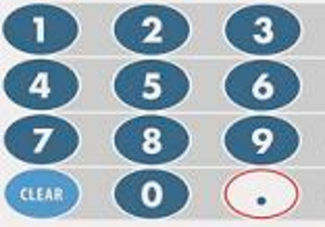
\includegraphics[scale=0.8]{images/background/numberpad.pdf}}
\caption{A number pad.}
\label{fig:numberpad}
\end{subfigure}
%\hfill%
\begin{subfigure}[b]{0.5\textwidth}
\centerline{
\includegraphics[scale=0.5]{images/background/incremental.pdf}}
\caption{An incremental interface.}
\label{fig:incremental}
\end{subfigure}

\caption[An incremental and keypad number entry interface.]{Two different number entry interfaces tested in \citeauthor{Oladimeji2011}'s study.}

\label{fig:interface-styles}
\end{center}
\end{figure}

Results of the study showed that a number keypad allowed people to enter a number more quickly than an incremental interface, but more errors were made. With the keypad, the visual attention was more on the input keys than the display. In an incremental interface, people were changing an existing value rather than entering a new value, so they had to look at the display to see how their actions changed the current value. This attention on the display may have made it more likely for them to detect errors in time. While an incremental interface may not be feasible when entering large amounts of data as it will slow users down too much, it may be preferrable over a keypad in situations where accuracy is of great importance \citep{Thimbleby2011}. 

In order to reduce human data entry errors, attempts have also been made to eliminate the need to manually enter data altogether. This is however not always possible, and moreover can introduce different problems.
\citet{Koppel2008} studied medication bags with a scannable bar code to enter numbers, so that the numeric values did not have to be typed by a person. They identified 31 workarounds if the system failed, for example if the bar code was missing, blurry or when the scanner did not work properly. Furthermore, even with a scanner numbers still have to be entered manually at some point, and it abstracts the numbers, which means users do not have a sense anymore of the magnitude of the numbers they are copying \citep{Wiseman2013a}. 

\subsubsection{Summary}
At the third stage of the data entry task, the user inputs the data into a device. Data entry has a speed-accuracy tradeoff, and being able to enter data faster often come at the cost of an increased error rate. 
Keyboards that slow people down may be useful in cases where accuracy is important, but may not be feasible in situations where a lot of data has to be entered. Depending on what users have to enter, shortcuts may get introduced in keyboard design so commonly used data can be entered quicker without the cost of increased errors. 

\subsubsection{The checking stage}
Most data transcription models consider the execution stage as the final stage of a data entry task \citep{Card1983, Salthouse1986}, but an additional stage can be a checking stage, where people review their entered output and compare it with the original target input, to see if it matches. 
In addition to studies trying to prevent errors before they occur, other studies have taken a different approach and looked at how a user can detect and correct errors after they have occurred. 

\subsubsection{Double data entry}
A number of studies have compared two or more of the following error checking techniques in data entry: visual checking, read aloud, and double data entry \citep{Barchard2011, Barchard2013, Kawado2003}. In visual checking, the user visually compares the entered data with the original data. In read aloud, data from the original source is read out loud by one user and the entries are visually checked by another user. In double data entry, data is entered twice and cross-checked by the computer system. 

Overall, double data entry is shown to be the most effective method in detecting errors. This method is often used in online forms when a user has to enter a password or e-mail address twice. The reasoning is that it is unlikely the same mistake is made twice. It is also not necessary for a system to know the correct input beforehand to determine if an entry error is made or not, because the two entries are cross-checked and if they do not match, an error has been made. 
 A disadvantage of double entry is that it requires double labour and can be time-consuming. Double data entry may therefore not be feasible for each setting. 
For example, \citet{Kawado2003} looked at copying medical data, and in their study 104,720 data entry fields had to be entered twice by two different people. In this study, the total times for double data entry was 74.8 hours while for the read aloud, where one person said the numbers and another person entered them, it was 57.9 hours. In situations where a lot of data has to be entered, such as data entry clerk work, it may therefore not be feasible to have to enter all data twice.  Moreover, it is still possible that a mistake is repeated, even when the entry is done by two different people \citep{Nakata2014}. In \citeauthor{Kawado2003}'s (2003) study, 42 errors remained undetected with the double data entry method.

\subsubsection{Visual checking}
Another method to detect errors is for the users to visually check their entered data with the original data source. Visual checking is a popular method \citep{Tu2014}, but simply asking or relying on people to check is often ineffective \citep{Barchard2011, Nakata2014, Norman2002, Olsen2008}. It is particularly hard to visually check numeric data, because there is no top-down error detection: almost any order of digits is a legal number \citep{Lin2014, Nakata2014}. Users can use the context of a word to detect if it is invalid, for example when 'wrod' is typed instead of 'word'. For numbers, if 697 is typed instead of 679 this may be harder to visually spot because 697 still counts as a valid number. 

\citet{Wiseman2013a} looked at a number entry task, and used a checksum to detect number entry errors. This is an extra number, that is related to the other entered numbers in a way that it is sufficient to only check the checksum to determine if the input is correct, instead of checking each entry one by one. 
They used infusion pump parameters in their study, and users were asked to enter the medication volume to be infused and the rate of infusion. If these two numbers were entered, the computer could calculate how long the infusion would take, and this time was the third checksum number.
If the checksum was generated by the computer from the two numbers entered and this checksum had to be visually checked by the user, only 36\% of the errors were caught. If the third number had to be entered by the user as well, and it was checked by the computer against the other two numbers, all errors were caught but the time to complete the task was increased by 46\%. These results show that visual checking was ineffective, but that asking the user to enter extra data can cause a considerable amount of time.

\citet{Olsen2008} conducted a lab experiment in which he simulated an internet banking tool, and participants were asked to enter account numbers from a paper sheet into a computer. After participants had entered an account number, they were presented with a confirmation screen with the input, and users were asked to check their input on this screen before submitting. 
Participants confirmed 88 trials where they had entered an incorrect account number. In addition, in 178 trials the simulator changed people's input to another number and this incorrect number was presented on the confirmation screen. Only 5 of these 178 errors were detected and corrected. This large amount of incorrect confirmations again suggests users do not check properly, even if they are explicitly asked to do so. 

\subsubsection{Lockouts}
Given the limited effectiveness of confirmation screens \citep{Norman2002, Olsen2008}, some studies have supplemented these with lockouts, where users have to wait a short period of time before they are able to confirm and submit their input. 

\citet{Green2014} introduced a lockout in a patient order entry system in a hospital. Every time a physician made an order for a patient, a prompt appeared asking to double-check the identity of the patient, and the button to continue an order would be disabled for 2.5 seconds. The prompt reduced the error rate by 30\%, but the total time to complete ordering tasks was lengthened by 1.5 hours on average. 

\citet{Gould2015} studied a number entry task where after each number the submit button would be disabled for a number of seconds, and a text instruction to check input appeared on the input screen.  This lockout was an effective method in encouraging people to check and detect errors in a lab setting. When the study was replicated online, a short lockout made people detect errors as well but the longer the lockout duration was, the more likely people were to switch to doing other tasks, and not check anymore. This illustrates the importance of taking the task context into account, and that findings from controlled studies do not always directly translate to an applied setting. In situations where people are able to work on other tasks, a lockout has to be brief to be effective and not induce switching to other tasks \citep{Gould2015}. 

Similar switching behaviour was found by \citet{Katidioti2013}. They conducted a lab experiment where people had to copy information and were interrupted by chat messages. Participants were free to choose when they wanted to attend to the messages. When people were locked out in the copying task and had to wait 3 seconds before they could enter the information, they often switched to the chat message, which made them forget the information to copy and slowed them down in completing the task.

\subsubsection{Incentives}
Instead of making design changes to the interface, \citet{Li2015} investigated if people can be motivated to check by incentives. 
They conducted a data entry experiment and manipulated the compensation people received after the experiment. In one condition, participants received extra money if they completed the task error-free. In another condition, money was deducted from their compensation if they made an error. In the control condition they received the same compensation regardless of their performance. Adding rewards and punishments significantly changed people's checking behaviour: they made more frequent and longer checks when their payment depended on their performance, and this resulted in fewer errors. 

\subsection{Improving data entry interfaces}

\subsubsection{Summary}
After people have entered input, they can choose to check if what they have entered is correct. A popular method is visual checking, but people are poor at doing this, even if they are instructed to do so. It is possible to have people check, but the context needs to be considered. A lockout helped people check, but when possible to switch to other tasks people used the time to spend time on other tasks.


\section{Conclusion}
Data entry follows four stages, and there are multiple strategies to complete the task, some being more accurate or efficient than others. Studies have shown that changing the design of a data entry interface can affect and improve how we enter data, and that different information access costs affect how often people visit the source from which to look up and enter data.

It is not known yet how these data entry designs can be used in an office setting, where people have to manage multiple information sources with varying information access costs. Studies on office work have shown that work can be highly fragmented, and that people may often have to go in and out of several applications to complete their task. 
In order to design interactive systems that truly support this type of data entry task, it is necessary to get a detailed understanding of the task in this setting, how users manage subtasks of looking up information for the data entry task, and to what extent the costs to access required resources affect their strategies.